\documentclass[11pt,oneside]{scrbook}
\usepackage[a4paper,margin=2.4cm,marginparwidth=1.8cm,marginparsep=0.4cm]{geometry}
\usepackage{../common/rlstudy}
\usepackage[ruled,vlined]{algorithm2e}

\title{{\color{rlblue}\textbf{Week 19} \\ \Huge DPO and the Preference Zoo}}
\author{STUDY-RL --- a self-paced Deep RL curriculum}
\date{\today}

\begin{document}
\maketitle
\tableofcontents
\newpage

\chapter*{Learning objectives}
\addcontentsline{toc}{chapter}{Learning objectives}


% Teaching companion: a small example before the full lecture.
\noindent\textbf{Study companion.} Read \texttt{teaching\_guide.md} in this
folder for step-by-step examples, an analogy with its limits, and self-checks.
Then use \texttt{workbook.ipynb} to implement and vary the calculations.
\par\medskip

\begin{keyidea}
By the end of this lecture you will be able to:
\begin{enumerate}[leftmargin=*]
  \item Derive the DPO loss in one continuous chain of equalities,
        starting from the KL-regularised RL objective of week~18 and
        the Bradley--Terry preference model.
  \item Describe the $\Psi$PO family and place DPO, IPO, KTO, ORPO,
        SimPO, and CPO inside it.
  \item Choose between sigmoid, hinge, and squared link functions
        with awareness of the saturation pitfall.
  \item Reason about reference-model needs, length bias and $\beta$
        tuning for each variant.
  \item Implement every loss in 10--15 lines of PyTorch.
  \item Run a DPO vs.\ KTO vs.\ SimPO bake-off and interpret reward
        margin, win-rate, and length distribution.
\end{enumerate}
\end{keyidea}

\chapter{Motivation \& intuition}

\section{From PPO to DPO --- the one-paragraph version}

Week~18 left us with three uncomfortable facts. The classical RLHF
pipeline keeps \emph{four} models in memory; PPO is notoriously
sensitive to hyper-parameters; and the entire stage~2 effort to fit a
reward model exists only because we are about to use it as a
\emph{loss function} inside stage~3. \textsc{Rafailov, Sharma,
Mitchell, Ermon, Manning, Finn} (NeurIPS 2023, arXiv:2305.18290) made
the following stunning observation. The closed-form optimum of the
KL-regularised RL objective (Theorem 3.2, week 18) is
\[
\pi^\star(y \given x) =
  \frac{1}{Z(x)} \pi_{\text{ref}}(y \given x)\,
  \exp\!\left(\frac{r(x,y)}{\beta}\right).
\]
Inverting this for $r$,
\[
r(x, y) = \beta \log\frac{\pi^\star(y \given x)}{\pi_{\text{ref}}(y \given x)}
          + \beta \log Z(x).
\]
\emph{This means the reward model is implicit in the policy.} Plug
this expression into the Bradley--Terry likelihood, the partition
functions $Z(x)$ cancel (they depend only on $x$, not on $y$), and
the entire stage 2 + stage 3 of RLHF collapses to one supervised loss
on $\pi_\theta$. No reward model. No PPO. No value head. No
adaptive KL. Just gradient descent on a contrastive log-likelihood.

\begin{intuition}
Think of it as a change of variables. RLHF asks: ``learn $r$, then
learn $\pi$ to maximise expected $r$.'' DPO asks: ``parameterise the
implicit $r$ \emph{through} $\pi$ via $r = \beta\log(\pi/\pi_\text{ref})$,
then maximise the BT likelihood of the preferences \emph{directly}
in $\pi$.'' Same optimal $\pi^\star$, no detour.
\end{intuition}

\section{The zoo}

DPO is the keystone. The 2024--2025 ``zoo'' is a family of objectives
that all aim to be \emph{DPO without one of its problems}:

\begin{itemize}[leftmargin=*]
  \item \textbf{IPO} (\textsc{Azar et al.\ 2024}, AISTATS) replaces
        the sigmoid with a squared loss. DPO's sigmoid saturates as
        the implied probability tends to 1; IPO does not, so it
        cannot push $\beta$ to infinity on deterministic preferences.
  \item \textbf{KTO} (\textsc{Ethayarajh et al.\ 2024}) drops the
        \emph{pair} requirement. A Kahneman--Tversky prospect-theory
        utility lets us learn from unpaired ``thumbs-up / thumbs-down''
        signals.
  \item \textbf{ORPO} (\textsc{Hong et al.\ 2024}, EMNLP) folds SFT
        into the preference loss via an odds-ratio penalty and
        \emph{removes} the reference model entirely.
  \item \textbf{SimPO} (\textsc{Meng, Xia, Chen}, NeurIPS 2024)
        is reference-free and \emph{length-normalised}: the implicit
        reward is the \emph{average} (not the sum) log-prob over the
        response.
  \item \textbf{CPO} (\textsc{Xu et al.\ 2024}, MT-focused) does
        contrastive log-ratio + SFT NLL without a reference model.
        Halves memory.
  \item \textbf{sDPO / iterative DPO} (week~20) refreshes the
        reference policy along the way.
\end{itemize}

By the end of this chapter the reader should be able to look at any
new ``XPO'' paper and reverse-engineer the four design knobs:
(a) \emph{link function} (sigmoid, hinge, squared), (b) \emph{reference}
(yes/no/refreshed), (c) \emph{normalisation} (sum, average, odds),
and (d) \emph{auxiliary loss} (SFT NLL or none).

\chapter{Mathematical formulation}

\section{The DPO derivation, in full}

We start from week~18's KL-regularised objective at a fixed prompt
$x$ (the prompt expectation is a sum over a finite dataset and adds
nothing to the algebra):
\begin{equation}
J(\pi) = \E_{y \sim \pi}[r(x, y)] - \beta\, \KL(\pi \,\|\, \pi_{\text{ref}}).
\label{eq:obj}
\end{equation}

\begin{theorem}[DPO loss; \textsc{Rafailov et al.\ 2023}]
\label{thm:dpo}
Assume $\beta>0$, positive reference support for compared responses, finite normalisation, and a sufficiently expressive policy class. Let preferences follow the Bradley--Terry model
$\Prb(y_w \succ y_l \given x) = \sigma(r(x,y_w) - r(x,y_l))$, and let
$\pi^\star$ be the optimum of \eqref{eq:obj}. Define the
\emph{implicit reward}
\[
\hat r_\theta(x, y) \defeq \beta \log\frac{\pi_\theta(y \given x)}{\pi_{\text{ref}}(y \given x)}.
\]
Then the maximum-likelihood estimator of $\theta$ under the BT model,
parametrised through $\hat r_\theta$, minimises
\begin{equation}
\mathcal{L}_{\text{DPO}}(\theta) =
  -\E_{(x, y_w, y_l)}\!\left[\log\sigma\!\left(
    \beta\log\frac{\pi_\theta(y_w \given x)}{\pi_{\text{ref}}(y_w \given x)}
    -
    \beta\log\frac{\pi_\theta(y_l \given x)}{\pi_{\text{ref}}(y_l \given x)}
  \right)\right].
\label{eq:dpo}
\end{equation}
\end{theorem}

\begin{proof}
Step 1.\ From Theorem 3.2 of week 18,
$\pi^\star(y \given x) = \pi_{\text{ref}}(y \given x) e^{r(x,y)/\beta} / Z(x)$.
Taking logs and rearranging gives
\begin{equation}
r(x, y) = \beta \log\frac{\pi^\star(y \given x)}{\pi_{\text{ref}}(y \given x)}
           + \beta \log Z(x).
\label{eq:rstar}
\end{equation}
Step 2.\ Insert \eqref{eq:rstar} into the BT difference:
\begin{align*}
r(x, y_w) - r(x, y_l)
&= \beta\!\left[\log\tfrac{\pi^\star(y_w \given x)}{\pi_{\text{ref}}(y_w \given x)} - \log\tfrac{\pi^\star(y_l \given x)}{\pi_{\text{ref}}(y_l \given x)}\right] + \underbrace{\beta \log Z(x) - \beta \log Z(x)}_{= 0} \\
&= \hat r_\theta(x, y_w) - \hat r_\theta(x, y_l) \quad\text{(with $\pi_\theta = \pi^\star$).}
\end{align*}
Step 3.\ The BT log-likelihood is therefore
$\log\sigma(\hat r_\theta(x, y_w) - \hat r_\theta(x, y_l))$. The factor $\beta$ is already included in $\hat r_\theta$.
Step 4.\ Maximising the BT log-likelihood in $\theta$ is minimising
its negative, which is \eqref{eq:dpo}. \qed
\end{proof}

\begin{remark}
The cancellation of $Z(x)$ in step 2 is the whole trick. It works
because $Z$ depends \emph{only} on the prompt; pairwise comparisons
within a prompt are insensitive to a prompt-level additive constant
on the reward (recall the BT identifiability remark in week~18). If
you ever try to compare completions across \emph{different} prompts
using DPO scores, you are eating the partition functions raw and
your numbers are meaningless.
\end{remark}

\begin{pitfall}
A common misreading: DPO ``does not need a reward model.'' That is
true \emph{operationally} but misleading conceptually. The implicit
reward $\hat r_\theta$ is still there; the policy parameters
\emph{are} the reward-model parameters. Reward hacking and
overoptimisation re-appear in DPO as ``likelihood displacement''
(\textsc{Razin et al.\ 2024}): the policy can win on the BT loss by
pushing $\log\pi(y_l)$ far down without making $y_w$ a good
sequence. See the safety angle below.
\end{pitfall}

\section{Margin losses and IPO}

Keep two quantities distinct:
\[
 h_\theta = \log\frac{\pi_\theta(y_w\mid x)}{\pi_{\mathrm{ref}}(y_w\mid x)}
             -\log\frac{\pi_\theta(y_l\mid x)}{\pi_{\mathrm{ref}}(y_l\mid x)},
 \qquad \Delta\hat r_\theta=\beta h_\theta.
\]
DPO uses $-\log\sigma(\beta h_\theta)$.
The offline IPO objective used in this project's implementation is
\begin{equation}
 \mathcal L_{\mathrm{IPO}}=\E[(h_\theta-1/(2\beta))^2].
 \label{eq:ipo}
\end{equation}
For an isolated unconstrained pair, the square is minimised at the finite
raw log-ratio margin $h_\theta=1/(2\beta)$, or implicit-reward margin $1/2$.
Shared parameters and conflicting or cyclic comparisons generally prevent
all individual pairs from reaching their targets simultaneously; a unique
policy minimiser does not follow from the scalar square.

Azar et al.'s $\Psi$PO framework transforms population preference
probabilities. It should not be identified with an arbitrary empirical
margin-loss replacement. The useful teaching comparison here is narrower:
DPO's loss tends to zero as a separable pair margin grows without bound,
whereas IPO has a finite scalar target. Both depend on the choice of
reference, reward scale, data, and policy class.

\section{KTO --- prospect theory without pairs}

KTO (\textsc{Ethayarajh et al.\ 2024}) replaces the pairwise BT model
by Kahneman--Tversky utility on \emph{unpaired} binary feedback
$z \in \{+, -\}$:
\begin{equation}
\mathcal{L}_{\text{KTO}}(\theta) =
  \E_{(x, y, z)}\!\left[\lambda_z \cdot v\!\left(\beta\,(\hat r_\theta(x, y) - z_{\text{ref}})\right)\right],
\label{eq:kto}
\end{equation}
where $z_{\text{ref}}$ is a prospect-theory \emph{reference point}
(an estimate of $\E[\KL(\pi_\theta \| \pi_{\text{ref}})]$ on a disjoint
batch) and $v$ is a concave-on-gains, convex-on-losses utility ---
in the TRL implementation, $v(u) = 1 - \sigma(u)$ for desirable
samples and $v(u) = 1 - \sigma(-u)$ for undesirable, with weight
parameters $\lambda_+$ and $\lambda_-$ separately controlling
gain-asymmetry. The practical payoff: a thumbs-up / thumbs-down log
collected in production is now a usable training signal.

\section{ORPO --- monolithic, reference-free}

ORPO (\textsc{Hong et al.\ 2024}) drops the reference policy and fuses
preference learning with SFT in a single backward pass:
\begin{equation}
\mathcal{L}_{\text{ORPO}}(\theta) =
  \underbrace{\E[-\log\pi_\theta(y_w \given x)]}_{\text{SFT NLL on winners}}
  - \beta\,\E\!\left[\log\sigma\!\left(\log\frac{\mathrm{odds}\,\pi_\theta(y_w \given x)}{\mathrm{odds}\,\pi_\theta(y_l \given x)}\right)\right],
\label{eq:orpo}
\end{equation}
with $\mathrm{odds}\,p = p/(1 - p)$. The odds-ratio penalty is
chosen because the gradient of $\log(p/(1-p))$ stays well-behaved
near $p = 1$ (unlike the plain log-likelihood), and the SFT term
provides an absolute anchor (winners get more probable, not just
relatively).

\begin{remark}[Numerical note]
Computing $\log\mathrm{odds}$ in log-space requires
$\log(1 - e^{\log p})$ which underflows for $\log p \in [-10^{-3}, 0]$.
Use the Mächler trick:
$\log(1 - e^x) = \log(-\mathrm{expm1}(x))$ for $x > \log(1/2)$,
$= \log_1p(-e^x)$ otherwise.
See \texttt{losses.\_log1mexp}.
\end{remark}

\section{SimPO --- reference-free, length-normalised}

SimPO (\textsc{Meng, Xia, Chen}, NeurIPS 2024) is the maximally
ergonomic variant:
\begin{equation}
\mathcal{L}_{\text{SimPO}}(\theta) =
  -\E\!\left[\log\sigma\!\left(\frac{\beta}{|y_w|}\log\pi_\theta(y_w \given x)
                                  - \frac{\beta}{|y_l|}\log\pi_\theta(y_l \given x)
                                  - \gamma\right)\right].
\label{eq:simpo}
\end{equation}
The implicit reward is the \emph{average per-token log-likelihood};
$\gamma$ is a target margin (typically $1.0$). Three design
implications:
\begin{itemize}[leftmargin=*]
  \item Reference-free: $\pi_{\text{ref}}$ vanishes.
  \item Length-normalised: long bad sequences and short bad sequences
        get the \emph{same} loss-per-token penalty --- this is the
        fix for DPO's length bias.
  \item Calibrated margin: $\gamma$ provides a non-zero target
        margin, so SimPO does not push every chosen sequence to
        probability one.
\end{itemize}

\begin{pitfall}
SimPO's length normalisation can \emph{under-train} short answers.
If your dataset has very short ideal completions (e.g.\ ``Yes.''
in QA), SimPO may not push them above longer wrong completions
strongly enough. Mitigation: cap $\gamma$ small, or mix in an SFT
NLL term (which is essentially CPO).
\end{pitfall}

\section{CPO --- contrastive + SFT, no reference}

CPO (\textsc{Xu et al.\ 2024}) is what you get if you take ORPO and
replace the \emph{odds}-ratio with a plain log-ratio:
\begin{equation}
\mathcal{L}_{\text{CPO}}(\theta) =
  \E[-\log\pi_\theta(y_w \given x)]
  - \E[\log\sigma(\beta\,(\log\pi_\theta(y_w \given x) - \log\pi_\theta(y_l \given x)))].
\label{eq:cpo}
\end{equation}
A halfway house between SFT and DPO. Particularly strong in machine
translation, where the SFT signal is dominant and the contrastive
term provides discriminative polish.

\section{Cheat-sheet of design knobs}

\begin{center}
\small
\begin{tabular}{lcccc}
\toprule
\textbf{Variant} & \textbf{Link} & \textbf{Reference?} & \textbf{Normalisation} & \textbf{SFT aux?} \\
\midrule
DPO  & sigmoid  & yes & sum log-prob   & no \\
IPO  & squared  & yes & sum log-prob   & no \\
KTO  & sigmoid (Kahneman) & yes & sum log-prob & no \\
ORPO & sigmoid  & no  & log-odds       & yes \\
SimPO & sigmoid & no  & average log-prob & no \\
CPO  & sigmoid  & no  & sum log-prob   & yes \\
sDPO & sigmoid  & refreshed & sum log-prob & no \\
\bottomrule
\end{tabular}
\end{center}

\chapter{Algorithms}

\begin{algorithm}[H]
\SetAlgoLined
\DontPrintSemicolon
\KwIn{SFT policy $\pi_{\text{ref}}$; preferences $\{(x_i, y_w^{(i)}, y_l^{(i)})\}$}
\KwOut{aligned policy $\pi_\theta$}
$\pi_\theta \gets \pi_{\text{ref}}$ \tcp*{warm start from SFT}
\For{$\text{step} = 1, \ldots, S$}{
  sample a mini-batch of preference triples \;
  forward $\pi_\theta$ on $(x, y_w)$ and $(x, y_l)$ to get $\log\pi_\theta(y_\bullet \given x)$ \;
  \textit{if variant in \{DPO, IPO, KTO\}:} forward $\pi_{\text{ref}}$ likewise (no grad) \;
  compute variant-specific loss (DPO eqn\ \eqref{eq:dpo}, IPO \eqref{eq:ipo}, etc.) \;
  Adam step on $\theta$ \;
}
\caption{Generic DPO-family training loop.}
\label{alg:dpo}
\end{algorithm}

\paragraph{Complexity.} Each preference step requires two forwards
on $\pi_\theta$ (one for $y_w$, one for $y_l$) and, for
ref-using variants, two more on $\pi_{\text{ref}}$. No rollouts, no
critic, no separate reward model: this is the entire reason DPO is
4--8$\times$ cheaper than PPO in practice.

\section{A worked numerical example}

\paragraph{DPO step on one pair.}
Suppose at some point in training,
$\log\pi_\theta(y_w \given x) = -3.0$, $\log\pi_\theta(y_l \given x) = -5.0$,
$\log\pi_{\text{ref}}(y_w \given x) = -3.5$, $\log\pi_{\text{ref}}(y_l \given x) = -3.5$,
$\beta = 0.1$.
The implicit rewards are
$\hat r_w = 0.1 \cdot (-3.0 - (-3.5)) = 0.05$,
$\hat r_l = 0.1 \cdot (-5.0 - (-3.5)) = -0.15$;
the margin is $0.2$;
the DPO loss is $-\log\sigma(0.2) \approx 0.598$.

\paragraph{SimPO step on the same pair, with $|y_w| = 10$,
$|y_l| = 30$.} The average log-likelihoods are
$-0.30$ and $-0.167$; the SimPO margin (before $\gamma$) is
$\beta \cdot ((-0.30) - (-0.167)) = 2 \cdot (-0.133) = -0.267$, so
SimPO is currently \emph{losing} on this pair: the longer-reject has a
higher average log-prob than the shorter-chosen. With $\gamma = 1.0$,
the loss is $-\log\sigma(-0.267 - 1.0) = -\log\sigma(-1.267) \approx 1.515$
--- substantially larger than DPO's $0.60$.
This is exactly the length-bias signal: SimPO will work \emph{harder}
to pull short winners above long losers than DPO does.

\chapter{Implementation walkthrough}

The full project lives in
\href{run:./project/}{\texttt{project/}}; the highlights:

\begin{itemize}
  \item \texttt{project/losses.py} --- the six losses, each in 10--15
        lines, with annotated docstrings.
  \item \texttt{project/train.py} --- generic
        \texttt{train\_variant()} loop and a one-call
        \texttt{bakeoff()} that runs all six.
  \item \texttt{project/data.py} --- the same toy preference dataset
        as week 18, for a fair PPO-vs-DPO comparison.
\end{itemize}

\paragraph{The DPO loss (annotated).}
\begin{codebox}
\begin{minted}{python}
def dpo_loss(logp_w, logp_l, logp_ref_w, logp_ref_l, beta=0.1):
    lr_w = logp_w - logp_ref_w  # log ratio winner
    lr_l = logp_l - logp_ref_l  # log ratio loser
    return -F.logsigmoid(beta * (lr_w - lr_l)).mean()
\end{minted}
\end{codebox}

\paragraph{IPO --- the squared link (annotated).}
\begin{codebox}
\begin{minted}{python}
def ipo_loss(logp_w, logp_l, logp_ref_w, logp_ref_l, beta=0.1):
    lr_w = logp_w - logp_ref_w
    lr_l = logp_l - logp_ref_l
    return ((lr_w - lr_l - 1.0 / (2.0 * beta)) ** 2).mean()
\end{minted}
\end{codebox}

\paragraph{SimPO --- reference-free, length-normalised (annotated).}
\begin{codebox}
\begin{minted}{python}
def simpo_loss(logp_w, logp_l, len_w, len_l, beta=2.0, gamma=1.0):
    avg_w = logp_w / len_w.clamp(min=1).float()
    avg_l = logp_l / len_l.clamp(min=1).float()
    return -F.logsigmoid(beta * (avg_w - avg_l) - gamma).mean()
\end{minted}
\end{codebox}

\paragraph{ORPO --- odds-ratio + SFT (annotated).}
\begin{codebox}
\begin{minted}{python}
def orpo_loss(logp_w, logp_l, nll_w, beta=0.1):
    log_odds_w = logp_w - _log1mexp(logp_w)
    log_odds_l = logp_l - _log1mexp(logp_l)
    return nll_w.mean() - beta * F.logsigmoid(log_odds_w - log_odds_l).mean()
\end{minted}
\end{codebox}

\paragraph{TRL on Qwen-2.5-0.5B (24~GB GPU).} Once you have a
preference dataset on disk:
\begin{codebox}
\begin{minted}{python}
from trl import DPOTrainer, DPOConfig
from peft import LoraConfig

trainer = DPOTrainer(
    model="Qwen/Qwen2.5-0.5B-Instruct",
    ref_model=None,                       # set to None when loss_type='simpo'
    args=DPOConfig(
        loss_type="sigmoid",              # 'sigmoid'=DPO, 'ipo', 'kto_pair',
                                          # 'simpo', 'cpo', 'orpo'
        beta=0.1,
        max_length=512,
        per_device_train_batch_size=4,
        gradient_accumulation_steps=8,
        learning_rate=1e-4,
        bf16=True,
        output_dir="runs/dpo",
    ),
    train_dataset=ultrafeedback_subset,
    peft_config=LoraConfig(r=16, lora_alpha=32,
                            target_modules=["q_proj","k_proj","v_proj","o_proj"]),
)
trainer.train()
\end{minted}
\end{codebox}
A 500-step run on $\sim$2 k preference pairs from
\texttt{trl-lib/ultrafeedback\_binarized} converges in about 30
minutes on an RTX 4090.

\chapter{Empirical results}

\autoref{fig:loss}, \autoref{fig:margin} and \autoref{fig:acc} show
the bake-off on the toy preference dataset. All six variants drive
the pairwise accuracy from chance ($\approx 0.5$) toward $1.0$ in
80 steps, but they get there along very different trajectories:
\textbf{IPO} has the smoothest margin growth (its target is finite),
\textbf{SimPO} ramps fastest in pairwise accuracy (length-normalisation
provides a strong signal on the highly length-imbalanced toy data),
and \textbf{ORPO} shows the SFT-anchor effect of falling NLL on
winners before the contrastive term kicks in.

\begin{figure}[ht]
\centering
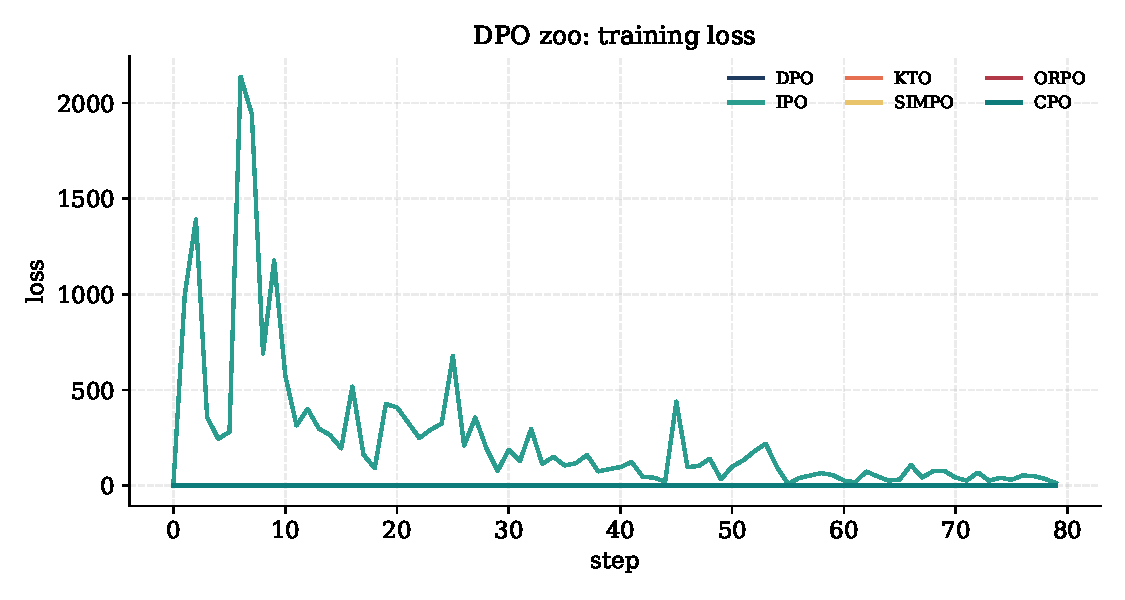
\includegraphics[width=0.95\linewidth]{figs/fig_loss.pdf}
\caption{Training loss for the six DPO-family variants on the toy
preference dataset, 80 steps from a common SFT checkpoint. Note that
loss values are \emph{not} directly comparable between variants
(different scales/normalisations); they are shown for sanity not
ranking.}
\label{fig:loss}
\end{figure}

\begin{figure}[ht]
\centering
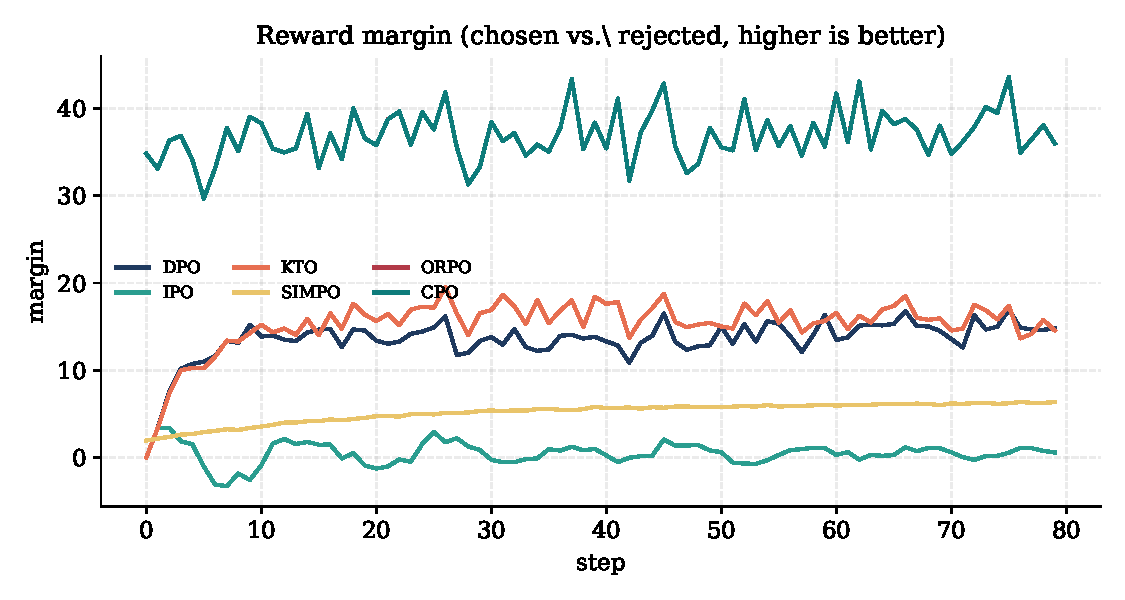
\includegraphics[width=0.95\linewidth]{figs/fig_margin.pdf}
\caption{Implicit reward margin (chosen minus rejected). Higher and
faster-growing is better; IPO targets a finite margin and plateaus,
DPO grows unboundedly.}
\label{fig:margin}
\end{figure}

\begin{figure}[ht]
\centering
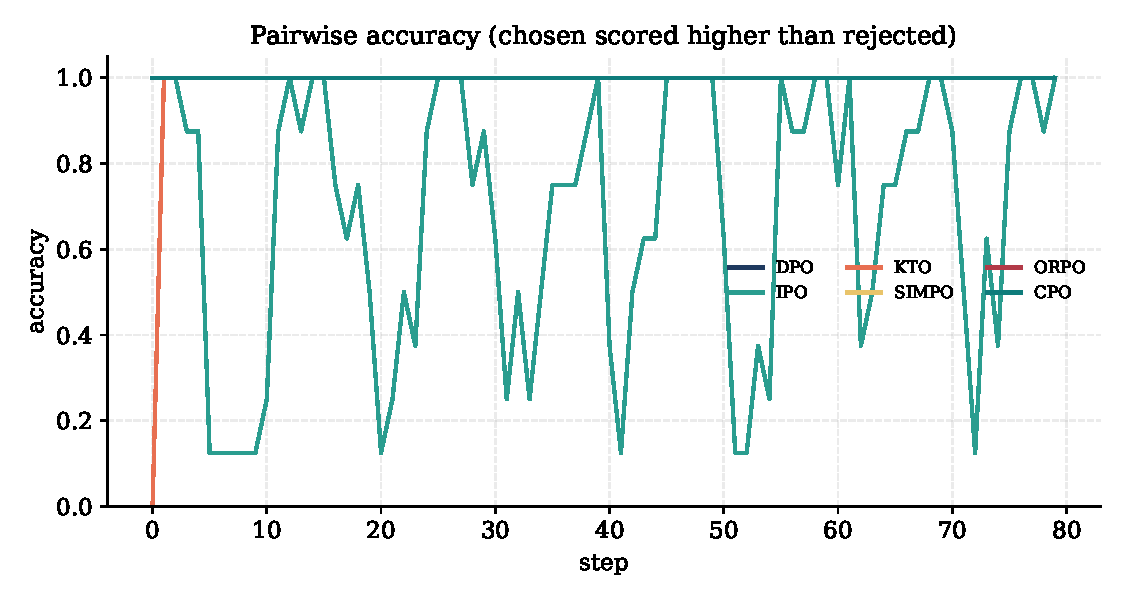
\includegraphics[width=0.95\linewidth]{figs/fig_acc.pdf}
\caption{Pairwise accuracy: fraction of preference triples on which
the chosen completion now scores higher than the rejected one.}
\label{fig:acc}
\end{figure}

\begin{figure}[ht]
\centering
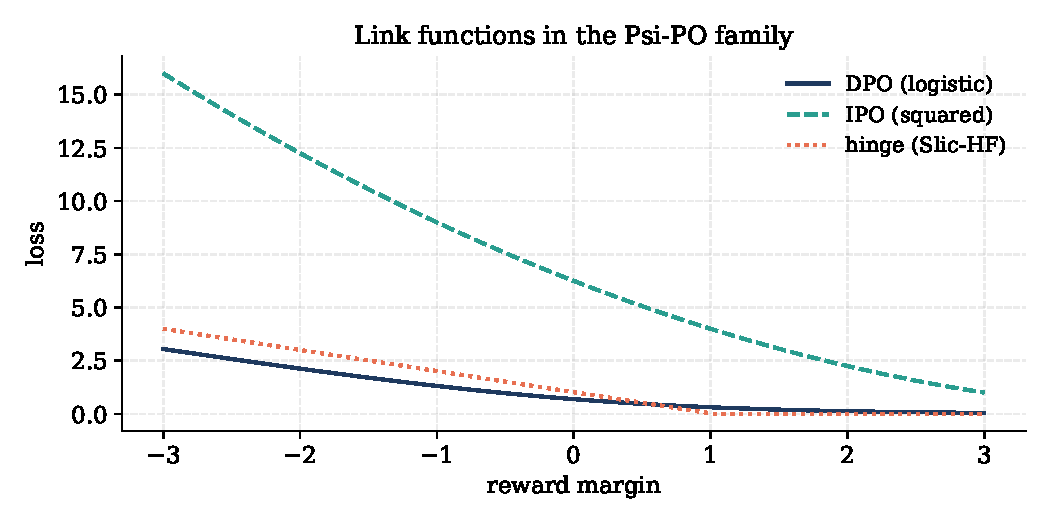
\includegraphics[width=0.85\linewidth]{figs/fig_links.pdf}
\caption{$\Psi$PO link functions, plotted against the reward
margin. The sigmoid saturates; the squared loss pins the margin to
a fixed target; the hinge is piecewise linear.}
\label{fig:links2}
\end{figure}

\paragraph{Notes on the bake-off.} The toy dataset is so easy that
all six variants reach near-perfect pairwise accuracy. On real data
(\texttt{ultrafeedback}, \texttt{hh-rlhf}, etc.) the ordering matches
the literature: SimPO and IPO tend to lead on AlpacaEval-2; ORPO is
strongest in low-resource one-stage settings; KTO is the only one
that works when you have no pairs. The toy bake-off here is meant to
demonstrate \emph{that the losses train at all} and let the student
inspect implementation details, not to rank methods.

\chapter{Theoretical deepening and FAQ}

\section{Why the partition function cancels (revisited, formally)}

The DPO derivation has one step that takes some getting used to:
$\beta\log Z(x)$ vanishing in the BT difference. Let us re-derive
this carefully.

\begin{lemma}[Pairwise invariance of BT]
\label{lem:bt-invariant}
For any function $c\!: \mathcal{X} \to \Real$ and any reward $r$,
the Bradley--Terry pairwise probability $\sigma(r(x, y_w) - r(x, y_l))$
is unchanged by the shift $r \mapsto r + c$.
\end{lemma}
\begin{proof}
$(r(x, y_w) + c(x)) - (r(x, y_l) + c(x)) = r(x, y_w) - r(x, y_l)$. \qed
\end{proof}

The same algebra applies to the maximum-likelihood estimator: any
$\log\sigma$-of-difference loss is invariant to a prompt-only
additive constant. The DPO derivation's $\beta\log Z(x)$ term is
such a constant. Hence ML estimation through the implicit-reward
parameterisation does not require us to compute $Z(x)$ ever.

\section{What is the implied reward model after DPO training?}

A subtle question. After $T$ steps of DPO, the implicit reward
$\hat r_\theta = \beta\log(\pi_\theta / \pi_{\text{ref}})$ is well-defined.
Is it close to a Bradley--Terry MLE on the preference data?

In the asymptotic limit (infinite data, exact gradient steps,
correct model class) -- yes. \textsc{Rafailov et al.} prove that
$\theta^\star$ minimising $\mathcal{L}_{\text{DPO}}$ corresponds to a
policy whose implicit reward is the BT MLE up to the prompt-level
constant.

In practice the equivalence is weaker. \textsc{Tang et al.\ 2024}
``Generalised Preference Optimization'' show that the gradients of
DPO differ from explicit-RM-then-RL gradients by an
\emph{importance-weight} factor. The two paths agree exactly only
on-policy.

\section{Why a fixed $\beta$ is a fragile hyper-parameter}

For a raw margin $h$, DPO has
$\partial\mathcal L/\partial h=-\beta\sigma(-\beta h)$.
At $h=0$, smaller $\beta$ therefore gives a smaller gradient magnitude,
not automatically faster training. In the ideal regularised optimum,
smaller $\beta$ permits more reward-driven drift. These are different
statements. In IPO the target $1/(2\beta)$ explicitly controls how far the
raw margin is pushed. Tune these parameters together with learning rate
using held-out preference quality, response lengths, and KL diagnostics.

\section{What preference data identifies}
At a fixed Bradley--Terry noise scale, connected preference comparisons
identify reward differences, not prompt-specific additive constants.
The policy regularisation strength $\beta$ expresses a reward--drift
trade-off; it is not determined by reference-policy likelihood differences
alone. There is no universal value of $\beta$ whose violation proves a bug.

\section{The DPO/SimPO ``win-rate gap'' explained}

A persistent empirical observation: SimPO posts higher AlpacaEval-2
length-controlled win rates than DPO at the same compute. Why?

Decompose AlpacaEval-2's ``length-controlled'' metric into raw
quality and a length-correlation correction. DPO trains on the
\emph{sum} log-prob, which has length-$|y|$-times the dynamic
range; the loss therefore rewards verbose winners more than
concise winners. SimPO normalises by length \emph{exactly}
matching the eval metric. So SimPO is, in a sense, ``tuned to the
benchmark''. The deeper claim --- that SimPO is also better in
human studies, not just on AlpacaEval --- is supported but not
ironclad.

\section{Q\&A: ten questions practitioners actually ask}

\begin{description}
  \item[Q1. Do I still need SFT before DPO?]
    Almost always yes. DPO from base inherits the base model's
    refusal patterns. Warm-start from SFT.
  \item[Q2. Do I need to keep $\pi_{\text{ref}}$ in fp32?]
    bf16 is fine for the reference. Numerical stability is dominated
    by the log-ratio difference, not the absolute log-probs.
  \item[Q3. Can I do DPO on completion-only loss (mask out the prompt)?]
    Yes, and you should. Including prompt tokens in the log-prob
    sum biases DPO toward long prompts.
  \item[Q4. Should I normalise the log-prob by completion length?]
    For DPO: only if you have length bias. For SimPO: that is
    the whole point. For IPO: not by default, but it helps.
  \item[Q5. Can I mix preference pairs from different sources?]
    Yes, but track per-source pairwise accuracy. Sources with
    contradictory preferences (one annotator pool prefers concise,
    another prefers verbose) will confuse the model.
  \item[Q6. How many pairs is ``enough''?]
    A few thousand for a 0.5--1.5B model; tens of thousands for
    7B--70B. Quality dominates quantity; \textsc{Tülu-3} uses
    $\sim$110k carefully curated pairs.
  \item[Q7. Can I combine DPO with RLVR?]
    Yes. \textsc{Tülu-3}'s recipe is SFT $\to$ DPO $\to$ RLVR-PPO.
    DPO does the preference polish; RLVR does the verifiable
    reasoning push.
  \item[Q8. Does DPO inherit reward hacking?]
    Not in the classical sense --- there is no reward model to hack
    --- but it inherits \emph{likelihood displacement}, which is
    behaviorally similar.
  \item[Q9. Why does IPO seem better in some papers and worse in others?]
    IPO shines when preferences are noisy or partially saturated;
    DPO shines when preferences are clean and the model has room
    to grow. The community consensus in 2026 is ``try both, IPO
    is more robust''.
  \item[Q10. Should I use iterative DPO?]
    For production, yes --- distribution shift is real and the
    single-shot DPO loss does not see it. Two or three iterations
    typically capture most of the benefit.
\end{description}

\section{A second worked numerical example: SimPO step}

Take the same toy completion as in our earlier walked example:
$\log\pi_\theta(y_w \given x) = -2.5, \log\pi_\theta(y_l \given x) = -8.0$,
with $|y_w| = 5, |y_l| = 20$. SimPO with $\beta = 2.0, \gamma = 1.0$
computes
\begin{align*}
\bar\ell_w &= -2.5 / 5 = -0.5, \\
\bar\ell_l &= -8.0 / 20 = -0.4, \\
\text{margin} &= 2.0 \cdot (-0.5 - (-0.4)) - 1.0 = -1.2, \\
\mathcal{L} &= -\log\sigma(-1.2) \approx 1.46.
\end{align*}
So SimPO thinks this pair is \emph{going the wrong way} (the long
loser has a higher average log-prob than the short chosen), and
produces a strong loss to push the model in the right direction.
If the reference assigns equal sequence log-probabilities to the pair,
DPO with $\beta = 0.1$ would compute a positive
log-ratio gap of order $0.1 \cdot (-2.5 - (-8.0)) = 0.55$ and a
loss of $-\log\sigma(0.55) \approx 0.45$ --- much smaller.

This is exactly the length-bias mechanism in action: SimPO is much
more sensitive to a short-but-bad winner being beaten by a
long-but-okay loser. Whether that sensitivity helps or hurts
depends on whether the data exhibits the length pathology --- in
most production datasets, it does.

\chapter{Safety angle}

\begin{safetyangle}
The DPO zoo inherits week 18's failure modes and adds two of its
own. \emph{Likelihood displacement} (\textsc{Razin et al.\ 2024}):
DPO and friends decrease $\log\pi(y_l)$ as aggressively as they
increase $\log\pi(y_w)$, often more so. The result is a policy that
``forgets'' fluent-but-rejected completions, which can manifest as
catastrophic forgetting of skills present only in losers but not in
winners --- a particularly insidious failure when preference data is
noisy or biased.

\emph{Distribution shift.} DPO is trained on a static, off-policy
preference set. The implicit reward $\hat r_\theta$ is therefore
only as good as that set's coverage of the policy's own
distribution. As $\pi_\theta$ moves during training, the
preference data describes an increasingly stale region; the
``iterative DPO'' family (\textsc{Liu et al.\ 2024},
\textsc{2025 survey arXiv:2503.12854}) addresses this by
periodically regenerating preferences with the new policy and
re-anchoring the reference.

\emph{Length inflation.} Plain DPO inflates response length by 20--60\%
over the SFT baseline (\textsc{Liu 2024}, \emph{Iterative
Length-Regularized DPO}). \emph{Mitigation}: SimPO's
length-normalised reward; or add a length-penalty term to the
implicit reward; or use Dr.GRPO-style sum-not-mean accounting.

\emph{Reference-policy drift.} All ref-using variants assume
$\pi_{\text{ref}}$ stays fixed. If your reference is a checkpoint that
itself was trained badly --- e.g.\ over-RLHF'd before you started ---
its biases will propagate. sDPO and TR-DPO refresh the reference
along the way to avoid this.

For synthetic insurance's matching deployment, the most consequential is
\emph{likelihood displacement}: a router trained with DPO on
``broker A vs.\ broker B'' clicks may aggressively suppress
moderate-fit brokers --- and brokers are not interchangeable
commodities. Watch the bottom of the implicit-reward distribution
as carefully as the top.
\end{safetyangle}

\chapter{Matching application}

\begin{matching}
The bake-off framework here translates directly to a synthetic insurance
``broker-ranking polish'' pipeline. After an SFT-style cold start
(supervised on historical broker--lead pairings that converted), the
team has three reasonable choices: \textbf{DPO} for the case where
the historic conversion data is roughly on-policy with the planned
production behaviour; \textbf{KTO} if signal is dominated by
unpaired thumbs-up / thumbs-down from broker partners; or
\textbf{SimPO} for the cheap, ref-free, length-normalised baseline.
The ``length'' in SimPO maps to ``number of suggested broker
options'' --- exactly the inflation we want to suppress.

For synthetic ATS, the candidate's apply-or-skip signal is unpaired
(``did they apply, yes/no'') which makes KTO the natural fit; the
``$z_{\text{ref}}$'' prospect-theory reference point is a recently
deployed router's average $\KL$ from the SFT model, an estimable
quantity. A bake-off mirroring this week's would test KTO against
ORPO (one-stage, ref-free, attractive for our limited compute) and
SimPO (the cheapest, length-normalised), with the win-rate judge
being a held-out conversion model rather than an LLM judge.
\end{matching}

\chapter{Exercises}

\begin{enumerate}[leftmargin=*]
  \item ($\star$) Derive the implicit reward $\hat r = \beta \log
        (\pi/\pi_{\text{ref}})$ from the closed-form RLHF optimum.
        \begin{intuition} Solve eq.\ (10) of week 18 for $r$, then
        notice that $\beta\log Z(x)$ cancels in any pairwise difference.
        \end{intuition}
  \item ($\star\star$) Implement \texttt{dpo\_loss} from scratch.
  \item ($\star\star\star$) Implement \texttt{ipo\_loss} from scratch
        and explain why its minimiser does not saturate.
  \item ($\star\star$) Implement \texttt{simpo\_loss}.
  \item ($\star\star$) Implement a numerically stable
        \texttt{log1mexp(x)} for $x \le 0$.
  \item ($\star\star$) Implement \texttt{orpo\_loss}.
  \item ($\star\star$) Implement a tiny LM-as-judge win-rate function:
        given two arrays of judge scores, return the fraction won by
        the first.
  \item ($\star\star$) Implement the implicit-reward-margin
        diagnostic and verify it tracks training progress.
  \item ($\star\star\star$) \emph{Open-ended:} run the full bake-off
        and report a \emph{length-bias} diagnostic (mean tokens of
        chosen vs.\ rejected after training) for DPO, SimPO and
        ORPO. Discuss the ordering.
  \item ($\star$) \emph{Meaningful objective:} re-derive
        $\mathcal{L}_{\text{DPO}}$ for a \emph{ranked} (not pairwise)
        preference of $k$ items; this is the seed of Plackett--Luce
        DPO and the ATS multi-suggestion-ranking setting.
\end{enumerate}

\chapter{Notation, conventions, and pseudocode for every variant}

\section{Notation cheat sheet}

\begin{center}
\small
\begin{tabular}{ll}
\toprule
Symbol & Meaning \\
\midrule
$x$ & prompt (string of tokens) \\
$y_w, y_l$ & winning and losing completions \\
$\pi_\theta(y \given x)$ & policy probability of completion $y$ given prompt $x$ \\
$\log\pi_\theta(y \given x)$ & sum over tokens of $\log\pi_\theta(y_t \given x, y_{<t})$ \\
$\pi_{\text{ref}}$ & frozen reference policy (typically the SFT checkpoint) \\
$\hat r_\theta(x, y)$ & implicit reward $\beta\log(\pi_\theta(y \given x)/\pi_{\text{ref}}(y \given x))$ \\
$\sigma(u)$ & logistic sigmoid $1/(1+e^{-u})$ \\
$\beta$ & temperature (DPO/IPO/KTO) or scale (SimPO) hyper-parameter \\
$\gamma$ & SimPO target margin \\
$|y|$ & length of completion $y$ in tokens \\
$\KL(p \| q)$ & Kullback--Leibler divergence \\
$Z(x)$ & per-prompt partition function of the closed-form optimal policy \\
\bottomrule
\end{tabular}
\end{center}

\section{One-page pseudocode for each variant}

\begin{algorithm}[H]
\SetAlgoLined\DontPrintSemicolon
\KwIn{batch $(x, y_w, y_l)$; $\pi_\theta$, $\pi_{\text{ref}}$; $\beta$}
$\ell_w \gets \log\pi_\theta(y_w \given x)$;\quad
$\ell_l \gets \log\pi_\theta(y_l \given x)$ \;
$\ell_w^{\text{ref}} \gets \log\pi_{\text{ref}}(y_w \given x)$;\quad
$\ell_l^{\text{ref}} \gets \log\pi_{\text{ref}}(y_l \given x)$ \;
$\mathcal{L} \gets - \log\sigma(\beta((\ell_w - \ell_w^{\text{ref}}) - (\ell_l - \ell_l^{\text{ref}})))$ \;
\Return $\mathcal{L}$ \;
\caption{DPO step.}
\end{algorithm}

\begin{algorithm}[H]
\SetAlgoLined\DontPrintSemicolon
\KwIn{batch $(x, y_w, y_l)$; $\pi_\theta$, $\pi_{\text{ref}}$; $\beta$}
$d \gets (\ell_w - \ell_w^{\text{ref}}) - (\ell_l - \ell_l^{\text{ref}})$ \;
$\mathcal{L} \gets (d - 1/(2\beta))^2$ \;
\Return $\mathcal{L}$ \;
\caption{IPO step.}
\end{algorithm}

\begin{algorithm}[H]
\SetAlgoLined\DontPrintSemicolon
\KwIn{batch $(x, y, z)$ with $z \in \{+, -\}$; $\pi_\theta$, $\pi_{\text{ref}}$;
       $\beta$, $\lambda_+$, $\lambda_-$, running estimate $z_{\text{ref}}$}
$\ell \gets \log\pi_\theta(y \given x);\quad \ell^{\text{ref}} \gets \log\pi_{\text{ref}}(y \given x)$ \;
$d \gets \beta\cdot((\ell - \ell^{\text{ref}}) - z_{\text{ref}})$ \;
$\mathcal{L} \gets z \cdot \lambda_+ (1 - \sigma(d)) + (1 - z) \cdot \lambda_- (1 - \sigma(-d))$ \;
\Return $\mathcal{L}$ \;
\caption{KTO step (unpaired).}
\end{algorithm}

\begin{algorithm}[H]
\SetAlgoLined\DontPrintSemicolon
\KwIn{batch $(x, y_w, y_l)$; $\pi_\theta$; $\beta$}
$\ell_w, \ell_l \gets \log\pi_\theta(y_w, y_l \given x)$ \;
$\mathrm{lo}_w \gets \ell_w - \log(1 - e^{\ell_w})$ \tcp*{stable via log1mexp}
$\mathrm{lo}_l \gets \ell_l - \log(1 - e^{\ell_l})$ \;
$\mathcal{L} \gets -\ell_w - \beta \log\sigma(\mathrm{lo}_w - \mathrm{lo}_l)$ \tcp*{NLL + odds-ratio}
\Return $\mathcal{L}$ \;
\caption{ORPO step (one-stage, reference-free).}
\end{algorithm}

\begin{algorithm}[H]
\SetAlgoLined\DontPrintSemicolon
\KwIn{batch $(x, y_w, y_l)$; $\pi_\theta$; $\beta$, $\gamma$}
$\bar\ell_w \gets \ell_w / |y_w|;\quad \bar\ell_l \gets \ell_l / |y_l|$ \;
$\mathcal{L} \gets -\log\sigma(\beta(\bar\ell_w - \bar\ell_l) - \gamma)$ \;
\Return $\mathcal{L}$ \;
\caption{SimPO step (reference-free, length-normalised).}
\end{algorithm}

\begin{algorithm}[H]
\SetAlgoLined\DontPrintSemicolon
\KwIn{batch $(x, y_w, y_l)$; $\pi_\theta$; $\beta$}
$\mathcal{L} \gets -\ell_w - \log\sigma(\beta(\ell_w - \ell_l))$ \;
\Return $\mathcal{L}$ \;
\caption{CPO step (SFT + contrastive, reference-free).}
\end{algorithm}

\section{Memory accounting on a 24 GB GPU}

For Qwen2.5-0.5B with LoRA $r=16$ on QKVO and bf16 weights, the
per-variant peak VRAM is approximately:

\begin{center}
\small
\begin{tabular}{lcc}
\toprule
Variant & Ref policy in VRAM? & Peak VRAM (GB) \\
\midrule
DPO   & yes & 3.8 \\
IPO   & yes & 3.8 \\
KTO   & yes & 4.0 \\
ORPO  & no  & 2.4 \\
SimPO & no  & 2.4 \\
CPO   & no  & 2.4 \\
\bottomrule
\end{tabular}
\end{center}

The reference-free variants leave significantly more headroom for
longer sequences or larger LoRA ranks --- a real practical advantage
that compounds over a 500-step run.

\chapter{Historical context: from BT to iterative DPO}

\section{Pre-history: pairwise ranking before LLMs}

The Bradley--Terry model is from 1952 --- ``Rank analysis of
incomplete block designs''. It predates RL by decades and was used
through the 20th century to rank chess players, soccer teams, and
peer-reviewed manuscripts. Its appearance in RLHF is a re-discovery,
not an invention.

The closely related Plackett--Luce model (1959) extends BT to
$k$-way rankings. Exercise 10 of the workbook derives a
Plackett--Luce DPO loss; ranked-DPO and the multi-suggestion ATS
setting both live in this generalisation.

\section{The discovery of the closed form}

The closed-form optimum of the KL-regularised RL objective
(week 18, Theorem 3.2) is a result from \emph{maximum entropy RL}.
It appears in \textsc{Ziebart 2010} (max-ent inverse RL), in
\textsc{Haarnoja 2017} (energy-based RL), and in the soft-actor-critic
lineage. \textsc{Peters \& Schaal 2007}'s Reward-Weighted Regression
is essentially the same identity in a different costume.

What \textsc{Rafailov et al.} added was the inversion --- expressing
$r$ in terms of $\pi^\star$ --- and the recognition that this
expression cancels with the BT partition function. The result was
sitting in the literature for fifteen years; nobody had connected
the dots to the LLM-alignment problem.

\section{The 2024 explosion}

Between October 2023 and December 2024, the DPO zoo proliferated:

\begin{center}
\small
\begin{tabular}{lcl}
\toprule
Date & Method & Contribution \\
\midrule
May 2023 & DPO    & the closed-form derivation \\
Oct 2023 & IPO    & squared loss, no saturation \\
Jan 2024 & Self-Rewarding LM & DPO + LLM-as-judge \\
Jan 2024 & CPO    & SFT + contrastive, no reference (MT) \\
Feb 2024 & KTO    & prospect theory, unpaired signals \\
Mar 2024 & ORPO   & odds-ratio, one-stage, no reference \\
May 2024 & SimPO  & length-normalised, no reference \\
Jun 2024 & Iter-LR-DPO & iterative + length regularisation \\
Jul 2024 & sDPO   & stepwise reference refresh \\
\bottomrule
\end{tabular}
\end{center}

By late 2024 the field had converged on a stable hierarchy:
\textbf{SimPO} as the strongest reference-free single-stage baseline,
\textbf{DPO} as the reference for theoretical analysis, \textbf{KTO}
for the practical case of unpaired signal, and \textbf{iterative
DPO / sDPO} for closing the distribution-shift gap.

\section{Where DPO did not win}

DPO's reign was contested on one major front: reasoning. By 2025,
verifiable-reward RL (GRPO, RLOO, DAPO --- week 20) had emerged as
the dominant paradigm for math and code, with DPO relegated to a
``preference polish'' step at the start or end of the recipe.
Tülu-3 and DeepSeek-R1's training pipelines both use DPO once and
then dive into RLVR.

The lesson: DPO is fantastic for \emph{style, helpfulness, tone,
refusal} --- the genuinely subjective dimensions where pairwise
human preferences are the gold standard. It is the wrong tool when
you can write a verifier.

\chapter{Further reading}

See \texttt{extended\_reading.pdf} for annotated summaries of
\textsc{Rafailov 2023} (DPO), \textsc{Azar 2024} (IPO),
\textsc{Ethayarajh 2024} (KTO), \textsc{Hong 2024} (ORPO),
\textsc{Meng, Xia, Chen 2024} (SimPO), and \textsc{Liu 2024}
(iterative length-regularised DPO). Sourced from
\texttt{research/llm\_rl\_sota.md} §2 (the DPO zoo) and §6
(iterative / online DPO).

\end{document}
